\documentclass[12]{article}
\usepackage{graphicx}
\usepackage{amsmath}
\usepackage{subcaption}
\usepackage{caption}
\usepackage{cleveref}
\begin{document}
\title{Minkasi - a Light-Weight, Extendable Maxmimum-Likelihood Mapmaker}
\section{Introduction}

A wealth of experiments map the sky using detectors that suffer from
$\frac{1}{f}$ noise in the raw timestreams.  In instruments with
multiple detectors, this noise is often correlated between detectors.
A major challenge is converting such data into maps of the sky that 1)
are optimal (or nearly optimal), 2) are faithful representations of
the sky (having either a very well understood transfer function which
ideally is unity), 3) do not leak noise artifacts along the scan
direction(s) (striping), and 4) can account for instrumental
systematics as part of the mapmaking process.  Several techniques have
been developed to deal with this (destriping, filter-and-bin,
maximum-likelihood) which can generally be understood in the same
mathematical framework but making different assumptions about the
noise or about how to minimize $\chi^2$.  We here describe a new
pipeline, named minkasi \footnote{Which is short for either Mustang
  Ninkasi or minimal Ninkasi} for making maximum-likelihood maps in
the presence of possibly complicated noise.  The design goal of
minkasi is ease of installation, ease of use, and ease of
extensibility while maintaining relatively good performance.  It does
this by keeping the data and pointing information in RAM, making it
suitable for small to medium problems (on current-day clusters, a few
TB of data are straightforward to map).  It is mainly written in
python, with a few performance-sensitive routines pushed to C.  We
first describe the general mapping problem and how maximum likelihood
solves for the sky.  We then describe some of the particular choices
made for minkasi.  We then show examples of maps made with minkasi
before concluding.

\section{Mapping Formalism}

Trying to extract information from data is an age-old problem.  Gauss
brought the field into the modern era with his development of
least-squares fitting, first used to rediscover Ceres after it had
been found but astronomers had lost track of it (ref xxx).  In the
usual data modelling problem, we have that our observed data $d$
depend on true model parameters $m_t$ through some function $\mathrm{A}$, and
have additive noise $n$.  To be clear, $d$, $m_t$, and $n$ are all
vectors, with $d$ and $n$ the same length.  We usually have $m_t$
shorter than $d$ as well.  Mathematically, we have 
\begin{equation}
d=\mathrm{A}(m_t)+n
\end{equation}
.  Our problem is to try to uncover the model given the
data, the mapping between model and data, and some idea of the
statistics of the noise.  In general, the noise will not be correlated
with the true signal, so we also have
\begin{equation}
\left <d\right >=\mathrm{A}(m_t)
\end{equation}
The next step is typically to assume that the noise is Gaussian and
describable by a covariance matrix $\mathrm{N} \equiv \left <n n^T
\right >$ or $N_{ij}=\left <n_in_j \right >$.  While this is often not
true, the central limit theorem suggests it will eventually be true
enough.  In the case of mapping, this assumption is virtually required
for computational tractability.  With Gaussianity, we can now write
the likelihood of getting the observed data given a model\footnote{One
  straightforward though possibly tedious way of deriving the matrix
  form is to start with the likelihood for uncorrelated Gaussian data,
  and show that the matrix form is element-wise identical.  One can
  then introduce a rotation matrix, and show that the rotated noise matrix
  elements are the noise covariances of the rotated data.} $m$, which may
or may not corresond to the true parameters $m_t$:
\begin{equation}
\log(\mathcal{L})=-\frac{1}{2} \left (d-\mathrm{A}(m))^T\right )
\mathrm{N}^{-1} \left (d-\mathrm{A}(m) \right )
\end{equation}
By convention, we work wtih $-2\log(\mathcal{L})$ which is called
$\chi^2$:
\begin{equation}
\chi^2 \equiv -2\log(\mathcal{L})= \left (d-\mathrm{A}(m))^T\right )
\mathrm{N}^{-1} \left (d-\mathrm{A}(m) \right )
\end{equation}
The {\textit{maximum likelihood}} solution is the set of parameters
that maximizes the likelihood of getting the observed data given the
model paramters.  Due to the monotonicity of $\log$, this is
equivalent to minimizing $\chi^2$.  An important point is that in
practice we have considerable freedom to swap nuisance terms between
the noise matrix and additional component of the model.  As long as
$\chi^2$ is left unchanged, we will get the same non-nuisance part
of the model (see the Appendix for a proof).  Many different mapping techniques amount to taking
advantage of this flexibility in different ways.  An instance of this is
destriping, which puts the $\frac{1}{f}$ part of the noise into $m$,
in turn making the residual noise white, which speeds the minimization
of $\chi^2$ considerably.  We stress that the discussion so far is
quit general, covering everything from sky maps to polynomial fits to nonlinear
Levenberg-Marquardt fitting.

\subsection{Linear Mapmaking}
An important sub-class of models are those where the data depend
linearly on the model paramters.  This turns $\mathrm{A}$ into a
matrix, transforms Equation \ref{eqn:data_model} into
\begin{eqnarray}
\label{eqn:linear_model}
d=\mathrm{A}m_t + n
\end{eqnarray}
and enables us to write down the global minimum for $\chi^2$.
We then have 
\begin{equation}
\chi^2 = \left (d-\mathrm{A}m\right )^T \mathrm{N}^{-1} \left (
d-\mathrm{A}m \right )
\end{equation}
We can differentiate with respect to $m$ and, after grouping
numerically identical terms, we have
\begin{equation}
\nabla \chi^2 = -2\mathrm{A}^T \mathrm{N}^{-1} \left
(d-\mathrm{A}m\right )
\end{equation}
At the minimum of $\chi^2$, the gradient must equal zero, so we have:
\begin{equation}
\label{eqn:mapmaking}
\mathrm{A}^T \mathrm{N}^{-1} \mathrm{A}m = \mathrm{A}^T \mathrm{N}^{-1}
d
\end{equation}
This is known as the {\textit{mapmaking equation}} and our task is, by
hook or by crook, to solve it\footnote{Some authors (e.g. wmap xxx)
  have actually solved a non-symmetric version of this as a way of
  dealing with data that are expected to be too contaminated to be
  used in the solution but good enough to be used in the noise.  We
  restrict ourselves to the symmetric case, but will show techniques
  that can accomplish the same goal.}.  

\subsubsection{Bias}
Let us insert Equation \ref{eqn:linear_model} into the mapmaking
equation.  We then have
\begin{equation}
\mathrm{A}^T \mathrm{N}^{-1} \mathrm{A}m =\mathrm{A}^T \mathrm{N}^{-1}
\left ( \mathrm{A}m_t+n \right )
\end{equation}
Assuming invertibility, we can multiply on the left by $(\mathrm{A}^T
\mathrm{N}^{-1} \mathrm{A})^{-1}$, leaving
\begin{equation}
\label{eqn:bias}
m=m_t+ \left (\mathrm{A}^T                                                                                                                                                 
\mathrm{N}^{-1} \mathrm{A} \right )^{-1} \mathrm{A}^T\mathrm{N}^{-1} n
\end{equation}
If the second term averages to zero, then our fit parameters will be
{\textit{unbiased}}, in the sense that $<m>=m_t$, as desired.  Note
that we have not used the fact that $N_{ij}=\left < n_i n_j \right >$,
so our solution will in general be {\textit{optimal}} if we have the
true noise, but remain {\textit{unbiased}} as long as we solve
something of the form of Equation \ref{eqn:mapmaking}.  

This result is a major reason why mapmaking works as well as it does -
we almost certainly won't get the noise quite right, but we'll still
have a useful map.  It is worth considering just how forgiving the
process can be.  Take the case where we have misweighted half of our
data by a factor of 2, and we want to take the average.  For
simplicity, we can take the limiting case where we have 2 data points
$y_1$ and $y_2$ (the proof for many data points will follow along
identical lines).  In that case,  our estimate of the mean will be
$(y_1+2y_2)/3$ for data, which has variance$(1+4)/9 = 5/9$.  We
{\textit{should}} have taken $(y_1+y_2)/2$ which has variance
$(1+1)/4=1/2$.  So, the variance of our estimator divided by the
variance if we had done everything perfectly is
$\frac{5/9}{1/2}=10/9$.  Since the errors go like the square root of
the variance, our factor of two misweighting results in an increase in
the errors of just 5.4\%.  We stress that overweighting a small amount
of bad data can be far worse than underweighting a small amount of
good data; in mapping, as in much of life, ``When in doubt, throw it
out'' are wise words.

In practice, ensuring that we remain unbiased can require care, since
we don't have the true noise covariance.  Rather, we estimate the
noise from the data, and so if any sky signal remains in the data when
we estimate the noise, we can have $\left <\mathrm{N}^{-1} n \right >
\neq 0$.  A common case would be where a point source is in timestream
data, and the noise is estimated by taking the variance of the data.
Timestreams that happened to fluctuate high over the source would
apparently have larger variance than those that happened to fluctuate
low.  The low-fluctuating timestreams would then have higher weight,
and our solution would systematically suppress power.  Usual solutions
include minimizing the degrees of freedom in the noise model and
iterating over noise estimation, subtracting the map from one noise
model before estimating the next.

\subsubsection{Parameter Errors}
We can also use Equation \ref{eqn:bias} to work out the parameter
covariance matrix $\left < (m-m_t) (m-m_t)^T \right >$:
\begin{equation}
\left < (m-m_t) (m-m_t)^T \right >=
\left <\left (\mathrm{A}^T
\mathrm{N}^{-1} \mathrm{A} \right )^{-1} \mathrm{A}^T\mathrm{N}^{-1} n
\left ( \left (\mathrm{A}^T
\mathrm{N}^{-1} \mathrm{A} \right )^{-1} \mathrm{A}^T\mathrm{N}^{-1}
n\right )^T\right >
\end{equation}
Recalling that $(\mathrm{AB})^T=\mathrm{B}^T\mathrm{A}^T$ and noting
that $\left <n n^t \right > = \mathrm{N}$, we have:
\begin{eqnarray}
\left < (m-m_t) (m-m_t)^T \right > =
\left (\mathrm{A}^T \mathrm{N}^{-1} \mathrm{A} \right )^{-1}
\left (\mathrm{A}^T \mathrm{N}^{-1} \mathrm{A} \right )
\left (\mathrm{A}^T \mathrm{N}^{-1} \mathrm{A} \right )^{-1}\\
=\left (\mathrm{A}^T \mathrm{N}^{-1} \mathrm{A} \right )^{-1}
\end{eqnarray}
If we can explicitly form $\left (\mathrm{A}^T \mathrm{N}^{-1}
\mathrm{A} \right )^{-1}$ then we have the full parameter errors and
covariances.  If that is computationally intractable, we can still get
selected errors.  Since we had to solve 
$\left (\mathrm{A}^T \mathrm{N}^{-1} \mathrm{A} \right )m=\left
(\mathrm{A}^T \mathrm{N}^{-1} \right )d$ 
to get our solution, we must have a way of solving
$\left (\mathrm{A}^T \mathrm{N}^{-1} \mathrm{A} \right )m=b$ for
general $b$.  If we set $b$ equal to zero everywhere, except for a
single 1, then solving that system gives us the column of $\left
(\mathrm{A}^T \mathrm{N}^{-1} \mathrm{A} \right )^{-1}$ corresponding
to the non-zero entry of $b$, which gives us the full parameter
covariances for the selected parameter.  This could be useful if we
care far more about a small number of parameters, or as a way to build
preconditioners.  

\subsubsection{Iterative Solutions}
For most cases where we are solving for a pixellized map of the sky,
it is far too computationally expensive to solve the mapmaking
equation by explicitly forming $\mathrm{A}^T \mathrm{N}^{-1}
\mathrm{A}$ and inverting it.  For instance, Planck HFI all-sky maps
use HEALPIX (ref xxx) Nside of 2048.  With three polarizations, that
is 150 million pixels per map, and direct inversion would take
$\sim10^{25}$ floating point operations, equivalent to multiple
decades with a petaflop-class machine just to carry out the
inversion.  However, iterative matrix solving techniques, such as
(preconditioned) conjugate gradient (ref xxx), work very well in
practice.  In its simplest form, conjugate gradient solves
$\mathrm{A}x=b$ for postitive-definite matrix $\mathrm{A}$ (distinct
from the matrix that maps parameters into data) by minimizing the
residual in a series of search directions that are orthogonal under
multiplication by $\mathrm{A}$.  In practice, this effectively solves
for the components of $x$ corresponding to the largest eigenvalues of
$\mathrm{A}$, with more iteratios solving for increasingly smaller
eigenvalues.  Conjugate gradient has the happy property that a single
iteration will solve for the components to all eigenvectors with the
same eigenvalue, and so useful solutions can generally be obtained
with a number of iterations set by the condition number of
$\mathrm{A}$ rather than its size.  A somewhat less appreciated
benefit of conjugate gradient is that it does not try to solve for
components corresponding to zero eigenvalues of $\mathrm{A}$, and so
it will happily provide useful solutions to singular problems without
having to invoke, say, a pseudo-inverse.  The archetypal example of
this is a map with an unmeasured zero-point, such as is commonly the
case in CMB maps where the detector absolute zero-points are not
known.  Conjugate gradient tends to leave the mean level unchanged,
which is almost certainly the desired behavior.  Of course, care must
be taken when using iterative solutions that scales of interest have
converged.  

The convergence of conjugate gradient can usually be sped up with the
introduction of a preconditioner.  In preconditioned conjugate
gradient (PCG), we solve 
\begin{equation}
\mathrm{A}^{\dagger}\mathrm{A}x=\mathrm{A}^{\dagger}b
\end{equation}
This clearly is solved when $\mathrm{A}x=b$, but to the extent that
$\mathrm{A}^\dagger$ is ``close'' to $\mathrm{A}^{-1}$, then the
condition number of $\mathrm{A}^{\dagger}\mathrm{A}$ shrinks and
convergence is faster.  One common preconditioner is the white noise
weight in the map (the Jacoby preconditioner) which tends to work well
on small scales.  In the limit the data noise is white and we are
solving for a pixellated map, the Jacoby preconditioner solves the
full problem in a single PCG iteration.  In our experience, improving
on the Jacoby preconditioner is challenging and highly
problem-dependent.  

In mapping, we need to be able to apply $\mathrm{A}^T \mathrm{N}^{-1}
\mathrm{A}$ to a series of trial vectors to run PCG.  We can think of
the matrix multiply as taking the trial vector, converting it into
predicted data (since $<d>=\mathrm{A}m$, inverse-variance weighting
that model data, then projecting the inverse variance-weighted model
data back into a map.  Our desired solution is then the one that
produces the same inverse variance-weighted projected map that the
true data give when inverse variance-weighted and projected.  We can
generally break up the data into chunks that have noise correlations
within the chunk, but no noise correlations between chunks.  A
standard example would be all the data from a single frequency from a
telescope for some period of time - different detectors will see
atmosphere or telescope thermal fluctuations in common, but those
would not be correlated with data taken at a different time.  We refer
to these chunks of (typically) time-ordered data as TODs.  In
practice, there can often be small correlations across TODs (such as
atmospheric fluctuations that cross a time boundary), but we emphasize
that maps remain unbiased in the presence of ignored noise
correlations.  Once we break up our data into independent TODs, then
$\mathrm{N}^{-1}$ becomes block-diagonal, and the processing of the
TODs remains independent up until the final projection step.  Since
that is a linear operation, we can treat the TODs independently, and
carry out a single final summation over TODs of $\mathrm{A}^T
\mathrm{N}^{-1} \mathrm{A}m$. Since that final summation, in the limit
of many TODs, is usually orders of magnitude faster than the various
projection and noise filtering operations, mapmaking parallelizes
extremely well, as different TODs can be assigned to different
processes, which only need to communicate via a single reduction
operation at the end of each iteration.


\subsubsection{Generalized Mapping}

The mapmaking equation is completely agnostic about the form of
$\mathrm{A}$.  Similarly, the fact that maps are unbiased (up to
singularities in $\mathrm{A}^T \mathrm{N}^{-1} \mathrm{A})$) even in
the presence of noise misestimation does not depend on $\mathrm{A}$.
Consequently, any data processing/systematics removal that can be done
as part of the mapmaking will give an unbiased map, as long as
something of the form of Equation \ref{eqn:mapmaking} is solved.  No
such guarantee can be made if the data are preprocessed, including
seemingly mundane operations like gapfilling and fixing jumps in
timestreams.  Instead, we should solve for nuisance parameters at the
same time we solve for the map.  So, we should construct $\mathrm{A}$
to include these nuisance parameters and solve for a generalized map,
which includes more (potentially far more) than just a map of the
sky.  We refer to this generalized map, which may contain many
components, as a mapset.

Fortunately, in practice the generalized mapping can usually be
gracefully implemented.  An iterative solver like PCG needs to form
$\mathrm{A}^T \mathrm{N}^{-1} d$ and repeatedly apply $\mathrm{A}^T
\mathrm{N}^{-1} \mathrm{A}$ to a mapset $m$.  We can think of this as
a series of operators: $\mathrm{A}^T \mathrm{N}^{-1}d$ takes the data,
inverse-variance weights it, then projects that onto a map.  This
would be the (unnormalized) dirty map in radio astronomy.  Then our
desired solution is the map that, when projected into data, gives the
same dirty map as the actual data.  Happily, when applying
$\mathrm{A}^T \mathrm{N}^{-1} \mathrm{A}$ to a mapset, components of
the mapset that map onto a single TOD stay local to that TOD after
applying $\mathrm{A}^T \mathrm{N}^{-1}\mathrm{A}$.  When
parallelizing, nuisance parameters local to a TOD never need to be
shared across nodes, with the only communication required being the
reduction of a single dot product carried out as part of PCG.  We can
then add nuisance parameters as needed to describe the observed data
without having to concern ourselves with anything other than how they
map onto the data, and how the data map back onto the nuisance parameters.

\section{Implementation of Mapping in Minkasi}

As we have seen in the previous section, a wide range of analyses can
carried out in a single framework as long as it has the ability to
efficiently map a model onto data, map data back into a model, and
noise-weight the data.  We now describe some of the default data
structures, noise models, and generalized map classes used in
minkasi.  

\subsection{Data Classes}

Out of the box, minkasi is designed to work with time-ordered data
typical of bolometer arrays.  Each chunk of data corresponds to an
instance of the Tod class.  Each process groups its TODs into a single
instance of the TodVec class.  The heard of each TOD instance is a
dictionary (TOD.info) that contains information about the TOD.  Key
entries include 'dx' and 'dy' that contain pointing information, and
'dat\_calib', which contains the raw (assumed to be calibrated) data.
The data are assumed to be in an $n_{detector}$ by $n_{data}$ array,
with index zero corresponding to detectors, and index one to the time
samples.  The pointing arrays are assumed to be of the same size and
shape as the data.  Each TOD also has a unique identifier ('tag') that
minkasi uses to keep track of the TODs.  The TOD is instantiated with
a python dictionary that gets copied into the TOD, which greatly
simplifies using minkasi with new experiments.  Extra keys in the
dictionary, which might contain experiment-specific data, are
allowed.  Typically, TODs are then assembled into a TodVec instance,
which holds the TODs in a python list and has associated methods to
loop over operations on TODs.  

\subsection{Noise Modelling}

Creating a good noise model is as much art as science.  Useful noise
models for bolometer arrays need to be able to describe correlations
between samples separated in time (generally referred to as
$\frac{1}{f}$ noise, even when the behavior differs from
$\frac{1}{f}$), and correlations between samples from different
detectors.  These correlations can be quite complicated, as
atmosphere, readout electronics, instrument temperature drifts and the
like can all contribute.  The usual assumtpion, which minkasi makes,
is that the noise is stationary.  Under that assumption, Fourier modes
of different frequencies are uncorrerlated (ref xxx), though the
detector-detector correlations must still be treated.  Since
maximum-likeilhood maps remain unbiased even in the presence of errors
in the noise model, stationarity need only be approximately true to be
useful.  

Operationally, given an in put array of data, a noise model needs to
calculate the inverse variance-weighted data. In practice, several
decisions must be made that balance flexibility, speed, robustness
while accounting for the finite length of timestreams.  The default
minkasi noise model (minkasi.NoiseSmoothedSVD) first calculates the
eigenvectors $\mathrm{V}$ of 
the detector-detector covariance matrix $dd^T$, where $d$is the
$n_{det}$ by $n_{data}$ two-dimensional data array.  Minkasi then
rotates into this space $d'=\mathrm{V}d$, and then transforms each of
the rotated timestreams into Fourier space, divides by the power
spectrum, transforms back into real space, and finally rotates these
mode timestreams back into detector timestreams.  In practice, there
are subtleties associated with many of these operations, which we now
describe.  

\subsubsection{Detector Rotation}
A good noise model must take into account correlations between
detectors when those correlations are significant.  A simple but
useful model is that each detector has its own noise uncorrelated with
other detectors, and that one or more physically distinct noiselike
signals are seen by multiple detectors.  Atmospheric common-mode
signals, where each detector moves in nearly perfect lock-step with
all the others, are is one common case.  In fact, for many cases, a
noise model that assumes arbitrarily large common atmsophere plus
white detector noise may be acceptable (ref cottingham, hincks).  Figure
\ref{fig:mustang_atmosphere} shows two typical MUSTANG2 TODs and
how dominant the common mode is.  This model is natively
supported (minkasi.NoiseCMWhite) and can be useful when trying to
understand if other noise models are misbehaving.  

Sadly, detector correlations are often not as simple as a single
common mode.  Sub-array atmospheric structure, ground pickup, readout
electronics, and thermal drifts are common sources of correlation.
The simplest solution, which minkasi adopts, is to rotate into the
singular value modes.  While simple, there are several caveats. The
first is simply time - the operation count scales like
$n_{data}n_{detector}^2$, and so for large arrays can become
expensive.  For a few hundred detectors, this is not likely to
dominate run time, but for a few thousand it probably will.  

A more subtle issue is that the SVD model forces the rotated
timestreams to be orthogonal, in the sense that their dot products are
zero both in time and across the array.  However, there is no reason
to think this is generally the case.  Take a simple case where two
halves of an array are read out separately, plus common-mode noise.
Red noise in the readout would couple noise within the half-arrays but
not across.  In general, the noise powers spectra will differ amongst
the three sources of correlated noise.  SVD modes will form an
orthogonal basis that averages over frequency.  This is not optimal,
though, since these orthogonal modes do not actually line up with the
physically independent sources of noise.  If the true power spectra
differ, the effect will be that some frequencies will have positive
correlations between the modes and some frequencies will have
negative, but those correlations will be ignored.  If the underlying
power spectra are the same, this effect goes away (and in fact
suggests that one should prewhiten data based on detector white noise
levels, which can usually be estimated simply and robustly frrom the
data using some sort of high pass filter.  Ideally, the noise model
would be based on the physically distinct components, but teasing them
apart can be challenging.  Tools like indepndent component analysis
(ICA ref xxx) are designed to do just that, but the authors have had
limited success actually gettign ICA to work usefully.  The default
minkasi model behaves well in practice for the data on which we have
tested it, but we encourage users to invest in understanding their
noise.  We also take this opportunity to remind the reader that
detector correlations can also be treated in the solution set, which
may be the easiest path to a solution and has been successfully used
before (e.g. ref fowler et al. xxx).  

We also note that minkasi supports an ACT-type model (xxx Dunner et
al.) that assumes there are a small number of correlated modes.  For
computational efficiency, the underlying noise power spectra are
assumed to be piecewise constant, and the detectors are otherwise
uncorrelated.  This model scales much better to large arrays since the
effective rotation scaling goes from the $n_{data}n_{detector}^2$ in
the default model to $n_{data}n_{detector}n_{mode}$.  While minkasi
has not been designed for very large-scale jobs, this noise model
(minkasi.NoiseBinnedEig) is likely useful for those who would like
to.  We finally note that one could couple a fast rotation into a
possibly useful space, such as the sum and difference of
polarization-sensitive detector pairs, before looking for further
correlations.  We have not found this useful since the atmosphere
usually can be described by a small number of modes across the array,
and noise-filtering those modes does as well as (in our experience,
even slightly better than) explicit pair differencing, while also
allowing for the use of unpaired detectors in making polarized maps.
However, that is not necessarily a universally true statement, and
some experiments may find such a model useful.


\begin{figure}
    \centering
    \begin{subfigure}[t]{0.45\textwidth}
        \centering
        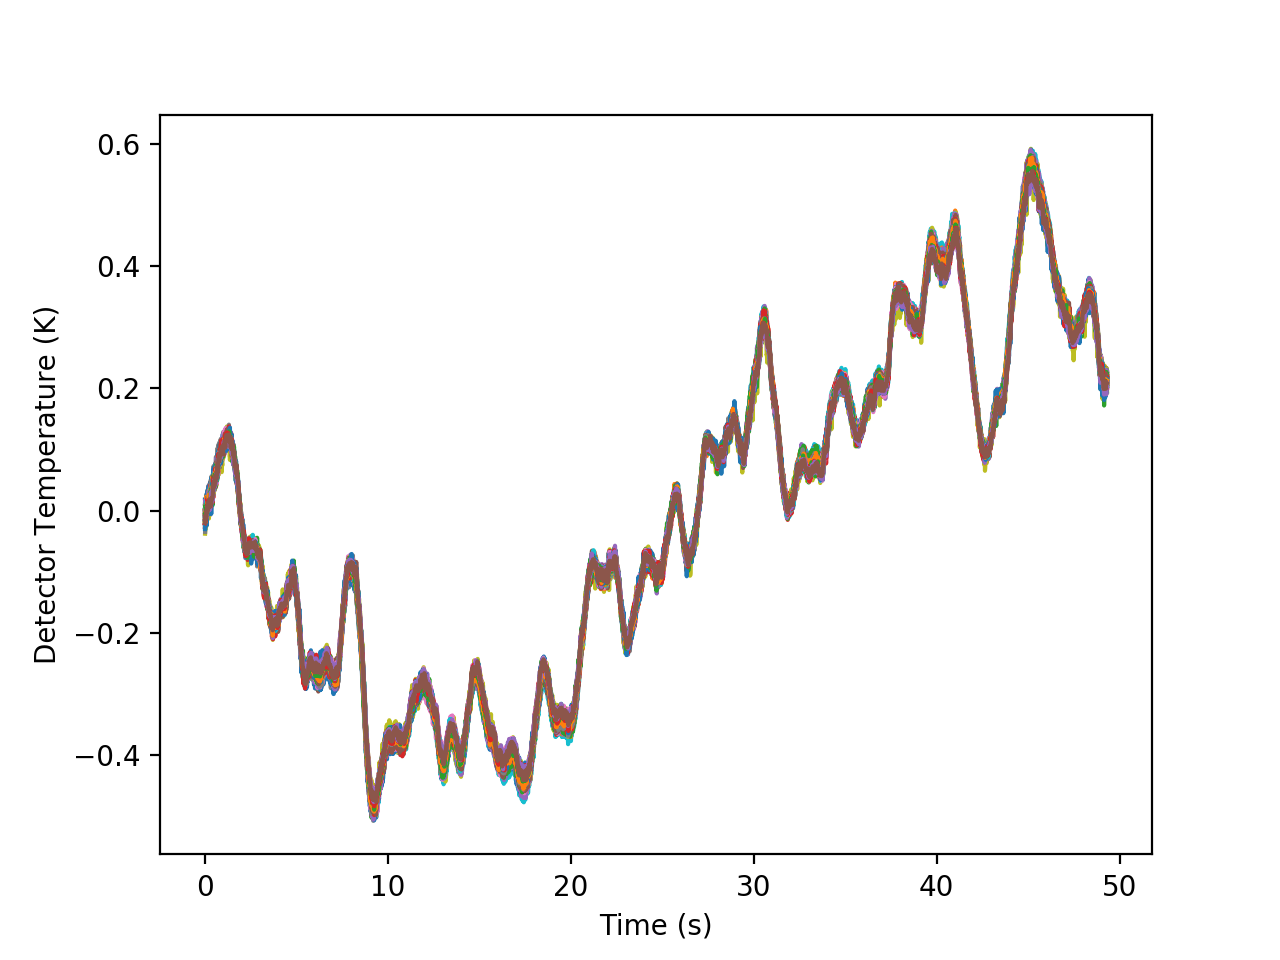
\includegraphics[width=\linewidth]{plots/all_detectors_AGBT18B_215_08-s60.png}
    \end{subfigure}
    \hfill
    \begin{subfigure}[t]{0.45\textwidth}
        \centering
        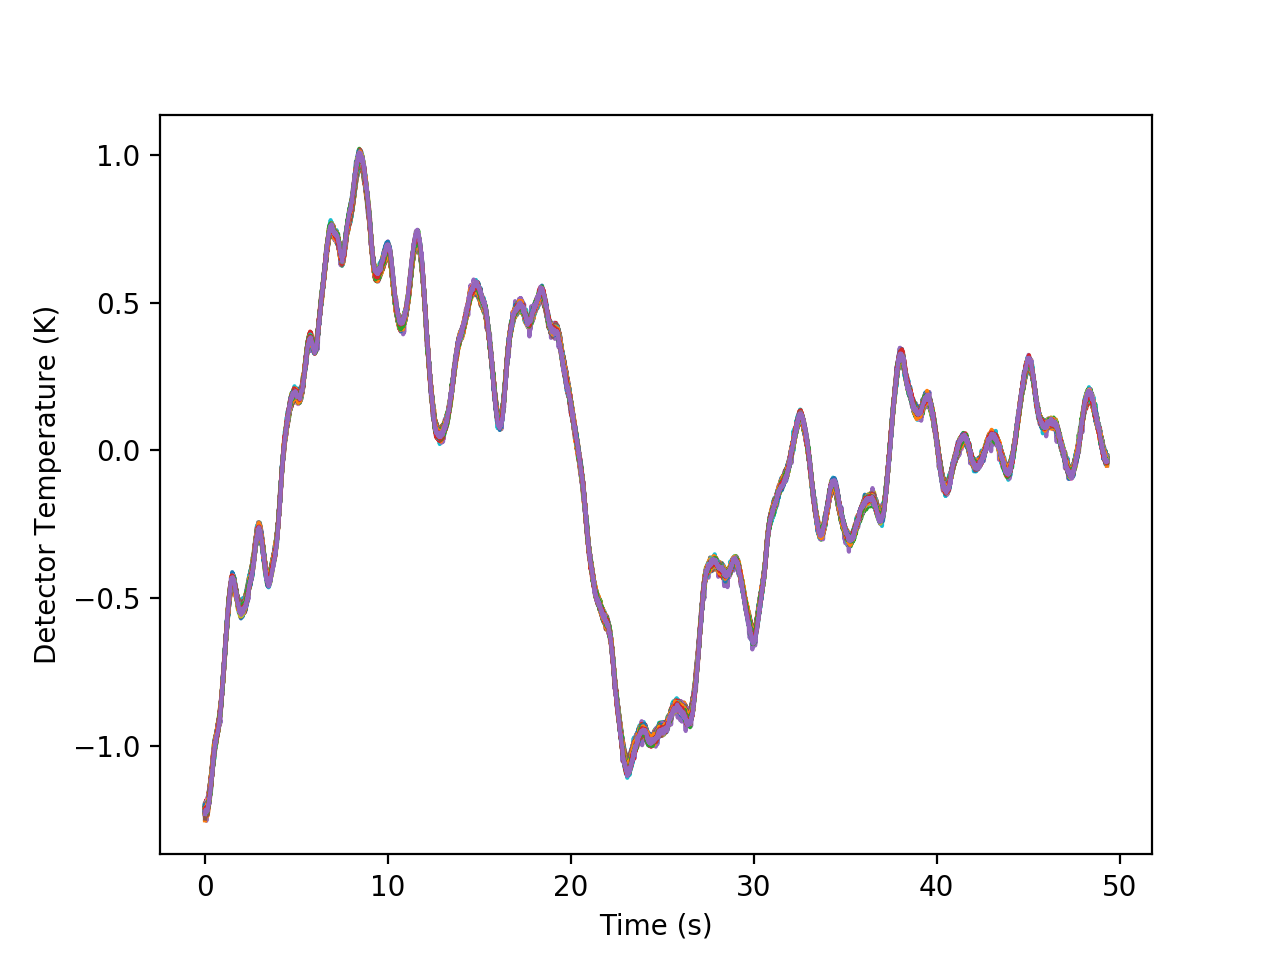
\includegraphics[width=\linewidth]{plots/all_detectors_AGBT18B_215_04-s101.png}
    \end{subfigure}
    \caption{Timestreams of all unflagged MUSTANG2 detectors for two random
      chunks of data.  Each plot has $\sim$150 detectors in it.  By
      far the dominant signal is common-mode atmosphere seen by all
      the detectors. Any good noise model must take this into account.}
    \label{fig:mustang_atmosphere}
    %(\subref{fig:timing1}) you can see a  green square....}
\end{figure}


\subsubsection{Fourier Transforms and Edge Effects}

Care must always be taken when applying discrete Fourier transforms to
non-periodic data.  To deal with edge effects, most codes apply a
window function before transforming.  This has the drawback of
downweighting data that have been windowed.  With windowing, one can
either accept the loss in sensitivty from downweighting otherwise good
data, or, at the expense of bookkeeping, overlap TODs by the width of
the window function.  The overlap method has the additional
complication of needing to handle detectors that were cut in one TOD
but not in an adjacent one.  Rather than dealing with window
functions, minkasi instead defaults to using real-to-real transforms
where the $n_{data}-2$ interior samples have been reflected in time
and appended to the the original data.  This has several nice
properties - the output transform is the same size as the input, and
up to an overall normalization, the forward and inverse transforms are
identical.  The main motivation, though, comes from the typical noise
encountered by ground-based instruments.  In the presence of a
long-term temperature drift, such as from the atmosphere, a standard,
non-windowed Fourier transform will pick up a $1/k$ component, or
$k^{-2}$ in the power spectrum.  Any noise component $k^{\alpha}$ with
$\alpha<-2$ would have higher frequencies be dominated by the leakeage
of power from low frequencies.  The real-to-real transforms, however,
turn the slope into a sawtooth pattern.  That Fourier transform scales
like $k^{-2}$, or $k^{-4}$ in the power spectrum. Atmospheric common
modes are frequently in the $\alpha={-8/3}$ to $\alpha=-11/3$ range one might expect
from integrating through a Kolmogorov$\alpha={-5/3}$ spectrum, so
one might expect for a broad class of ground-based data that the
real-to-real transforms can be used without windowing.  Figure
\ref{fig:noise_sims} shows the average power spectra from 1000
non-periodic simulations with low-frequency noise indices of
$\alpha=(-\frac{5}{3}, -\frac{8/3}, -5)$.  Spectra using standard fast
Fourier transforms (FFTs), real-to-real transforms, and windowed FFTs
are shown.  As expected, for $\alpha=-5/3$, power spectra from all
three methods agree with the true model.  For $\alpha=-8/3$, the
real-to-real and windowed FFTs agree with the model, but the plain FFT
does not.  For $\alpha=-5$, only the windowed FFT is correct.  While
the authors have not encoutered extremely red noise with $\alpha<-4$
in practice, we nevertheless stress that users should check this
before blindly using real-to-real transforms.  Over and above
estimating the power spectrum correctly, we also need to ensure that
edge effects do not show up in the noise-weighted data.  The final
panel of Figure \ref{fig:noise_sims} show the variance of
noise-filtered non-periodic timestreams for $\alpha=-5/3$.  The
windowed variance follows the shape of the window function.  The
standard FFT has a spike in variance at the edges, so even though for
this index the power spectra are correct, unwindowed FFTs still should
not be used without masking edges.  Happily, the real-to-real
transforms maintain constant variance across the full timestream for
$\alpha=-5/3$ and $\alpha=-8/3$ (but not for $\alpha=-5$, as
expected), and so we adopt unwindowed real-to-real transforms as the
default for minkasi.


\begin{figure}
    \centering
    \begin{subfigure}[t]{0.45\textwidth}
        \centering
        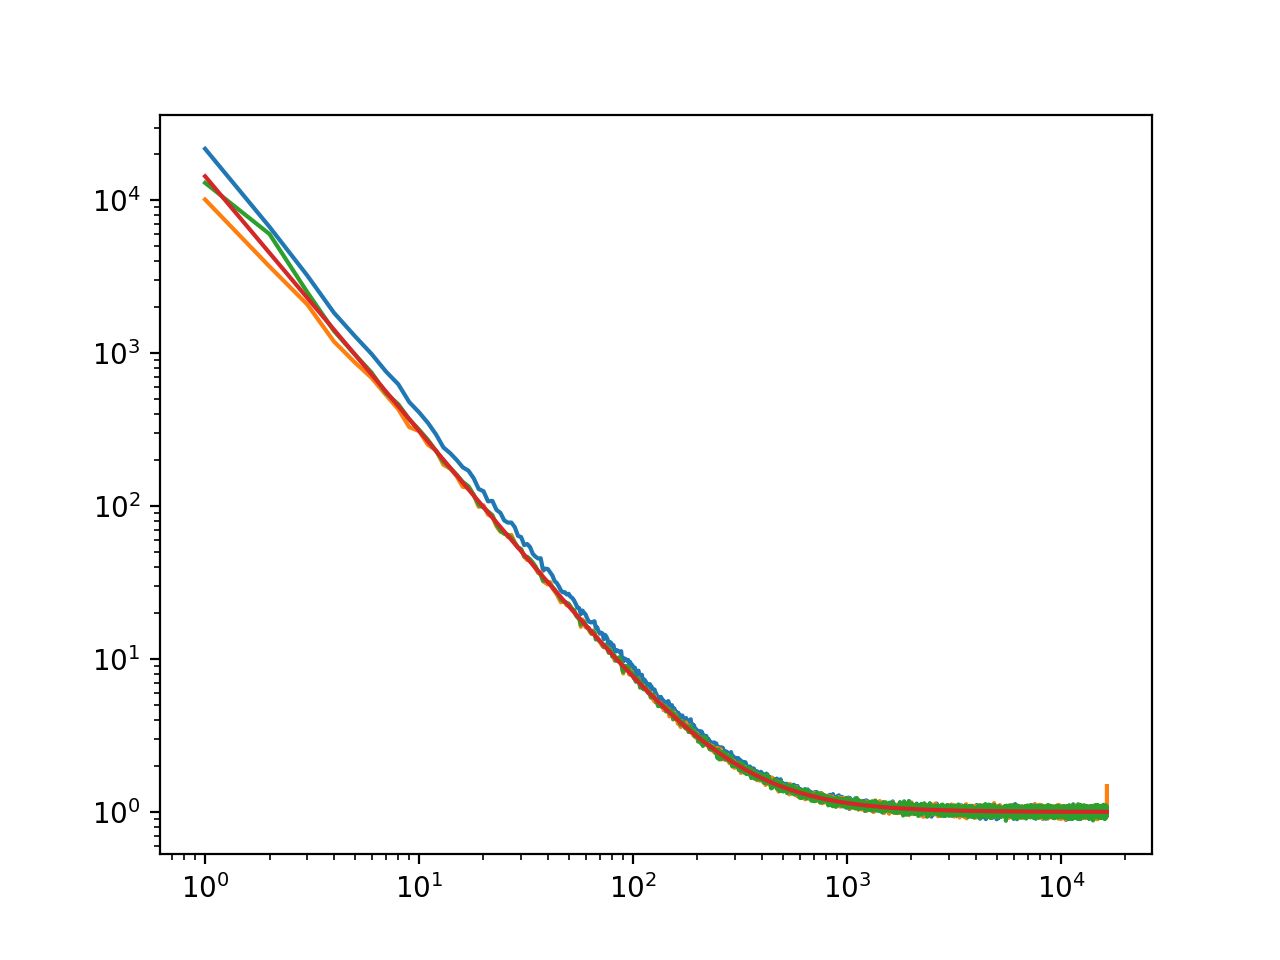
\includegraphics[width=\linewidth]{plots/power_spectra_5_3.png}
        %\caption{Generic} 
        %\label{fig:noise_sims}
    \end{subfigure}
    \hfill
    \begin{subfigure}[t]{0.45\textwidth}
        \centering
        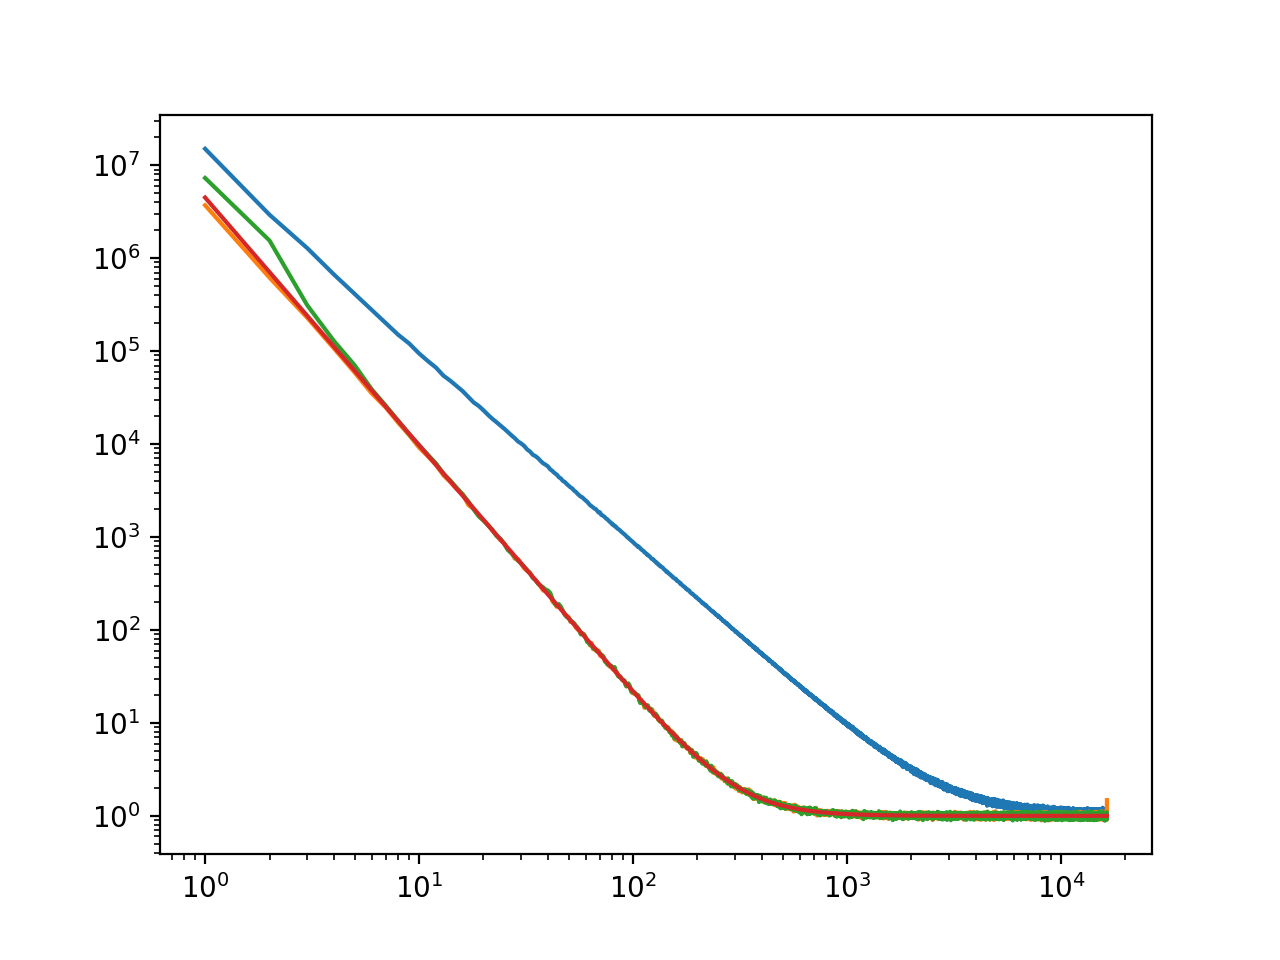
\includegraphics[width=\linewidth]{plots/power_spectra_8_3.png}
        %\caption{Competitors} \label{fig:timing2}
    \end{subfigure}

    \vspace{1cm}
    \begin{subfigure}[t]{0.45\textwidth}
    \centering
        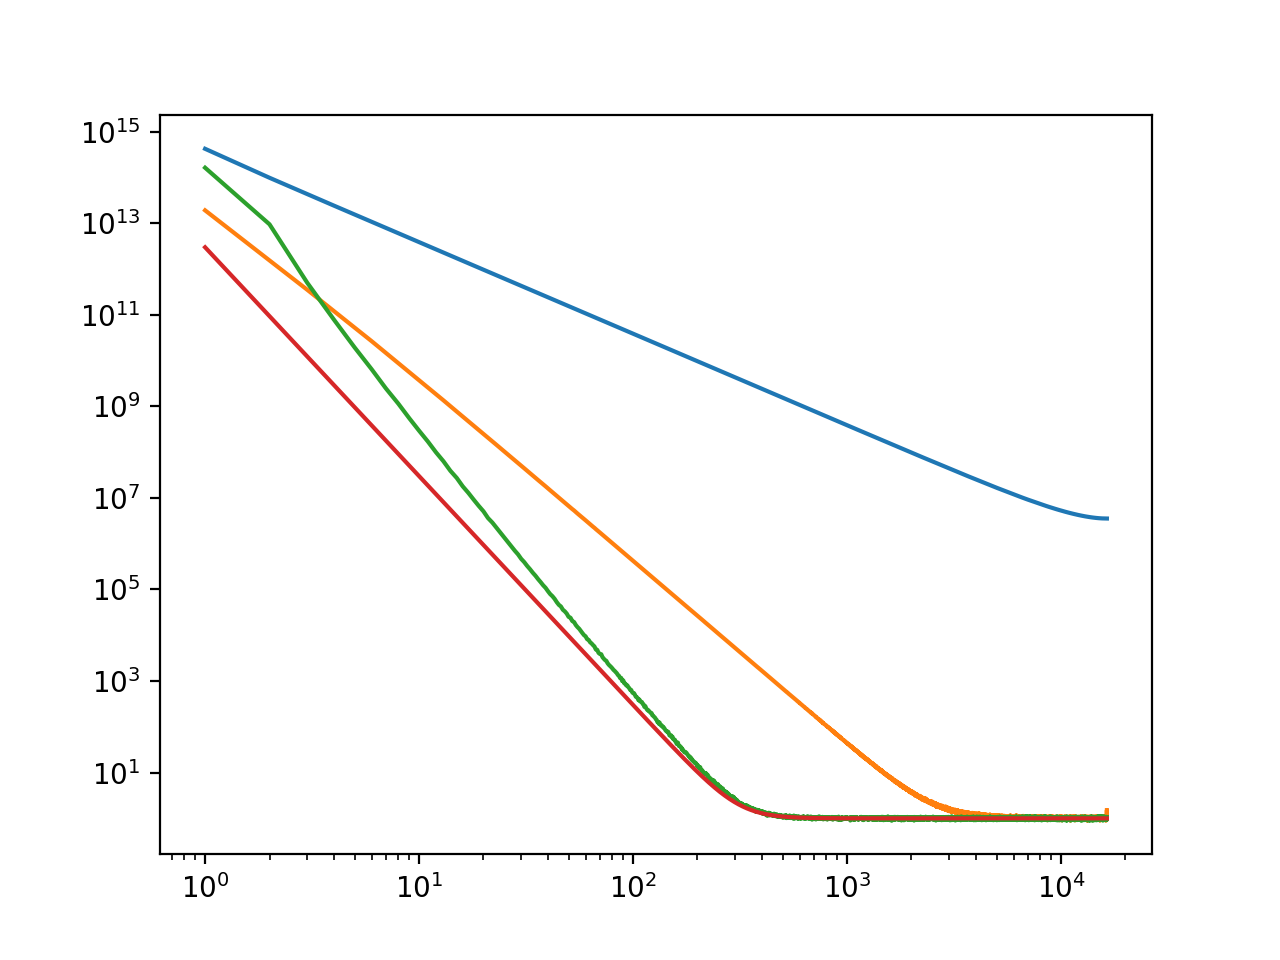
\includegraphics[width=\linewidth]{plots/power_spectra_5.png}
        %\caption{Price regulation} \label{fig:timing3}
    \end{subfigure}
    \hfill
    \begin{subfigure}[t]{0.45\textwidth}
      \centering
      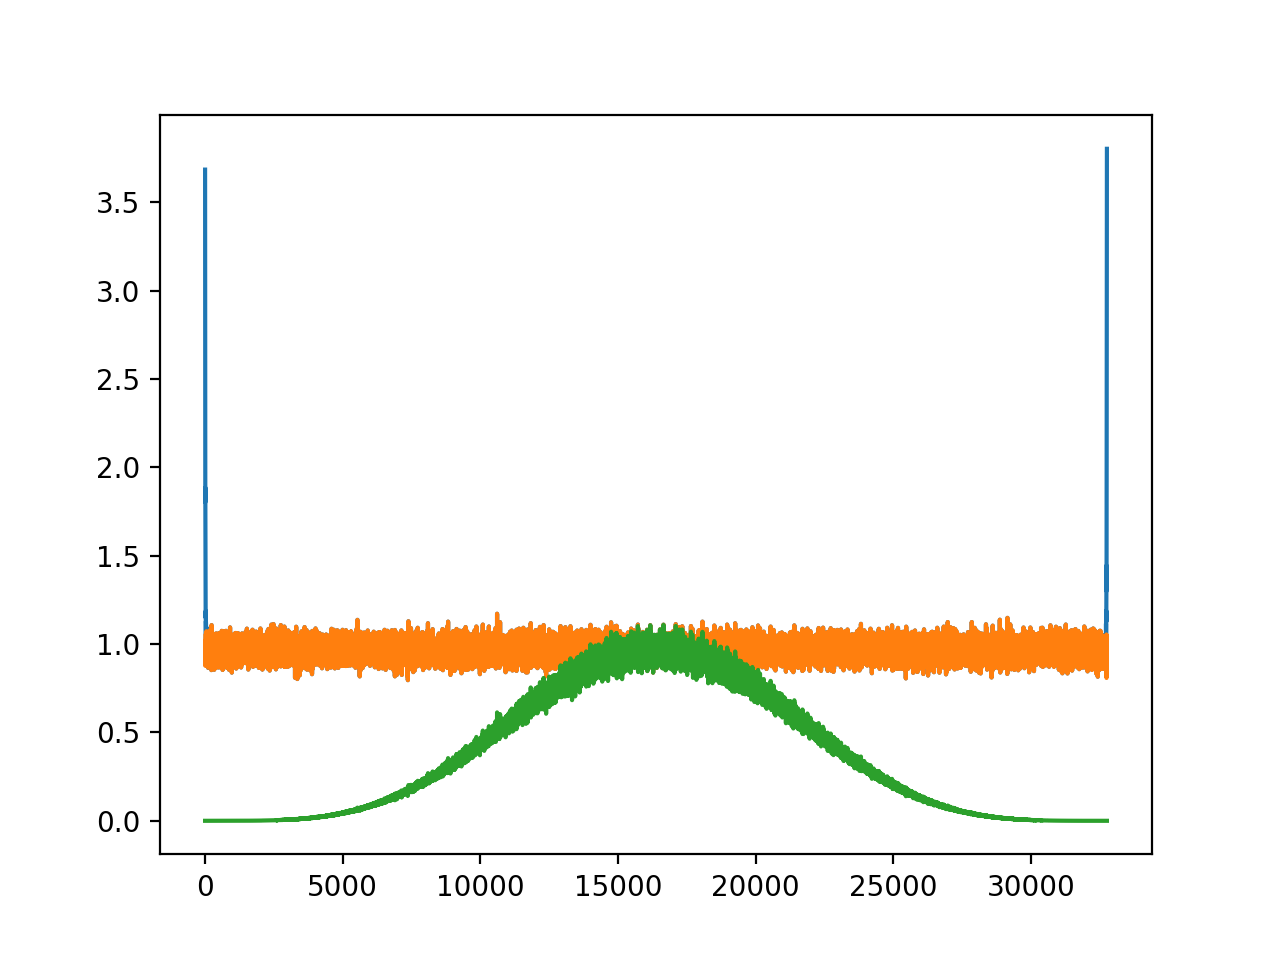
\includegraphics[width=\linewidth]{plots/filtered_variance_5_3.png}
      %\caption{Price regulation} \label{fig:timing3}                                                                                                                                                                    
    \end{subfigure}
    \caption{Power spectra of non-periodic timestreams with
      low-frequency indices of $\alpha=-5/3$ (top left), $\alpha=-8/3$
      (top right), and $\alpha=-5$ (bottom left).  The spectra are
      calculated using standard FFTs (blue), real-to-real transforms
      (orange), and windowed FFTs (green).  The input model is in
      red.  As expected, all three techniques produce correct power
      spectra for $\alpha=-5/3$, the standard FFT breaks down for
      $\alpha=-8/3$, and the real-to-real breaks down for
      $\alpha=-5$.  At $\alpha=-5$, even the windowed FFT begins to
      break down.  The bottom right shows the variance of the
      inverse variance-weighted timestreams using the three techniques
      for $\alpha=-5/3$.  Even though the power spectrum of the
      unwindowed FFTs are correct, edge effects remain in the variance
      which are not present for the real-to-real transforms.  This
      remains true for $\alpha=-8/3$ but, as expected, breaks down for
      $\alpha=-5$.}
    \label{fig:noise_sims}
    %(\subref{fig:timing1}) you can see a  green square....}
\end{figure}


%\begin{figure}[!h]
%  \centering
%  \begin{subfigure}{0.45\textwidth}
%  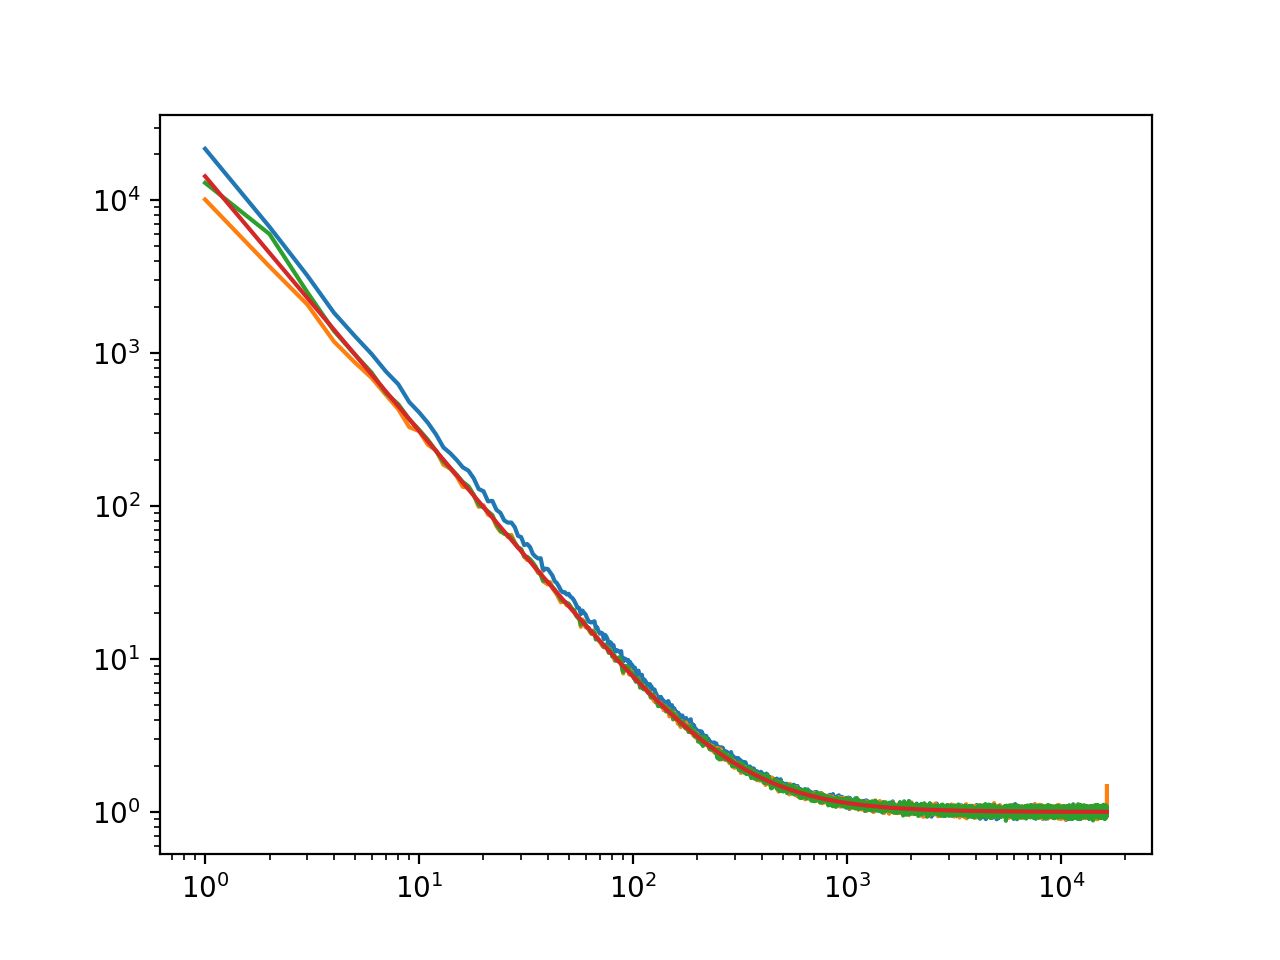
\includegraphics[width=\linewidth]{plots/power_spectra_5_3.png}
%  \end{subfigure}
%  \begin{subfigure}
%  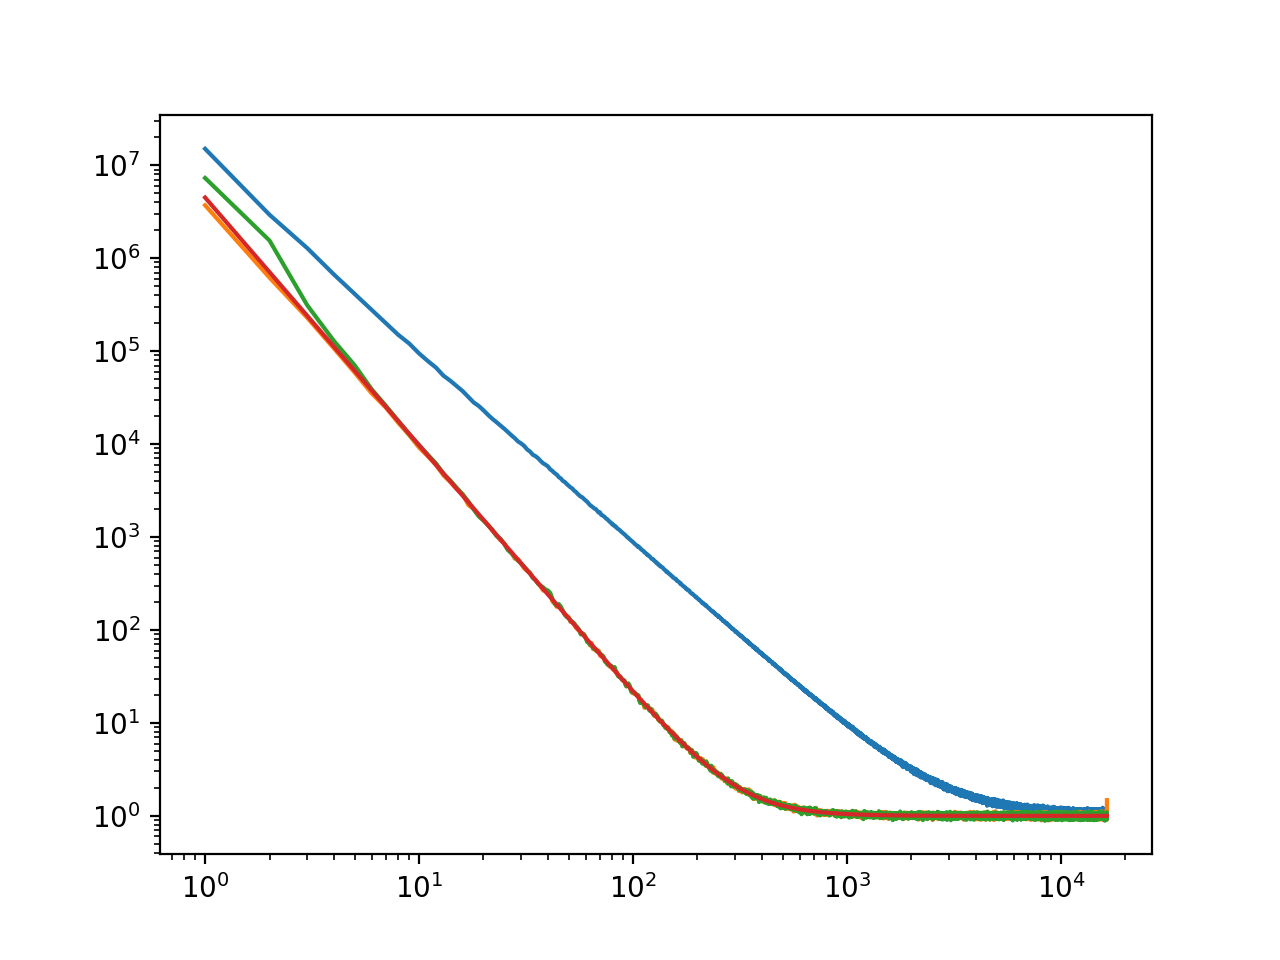
\includegraphics[width=\linewidth]{plots/power_spectra_8_3.png}
%  \end{subfigure}
%  %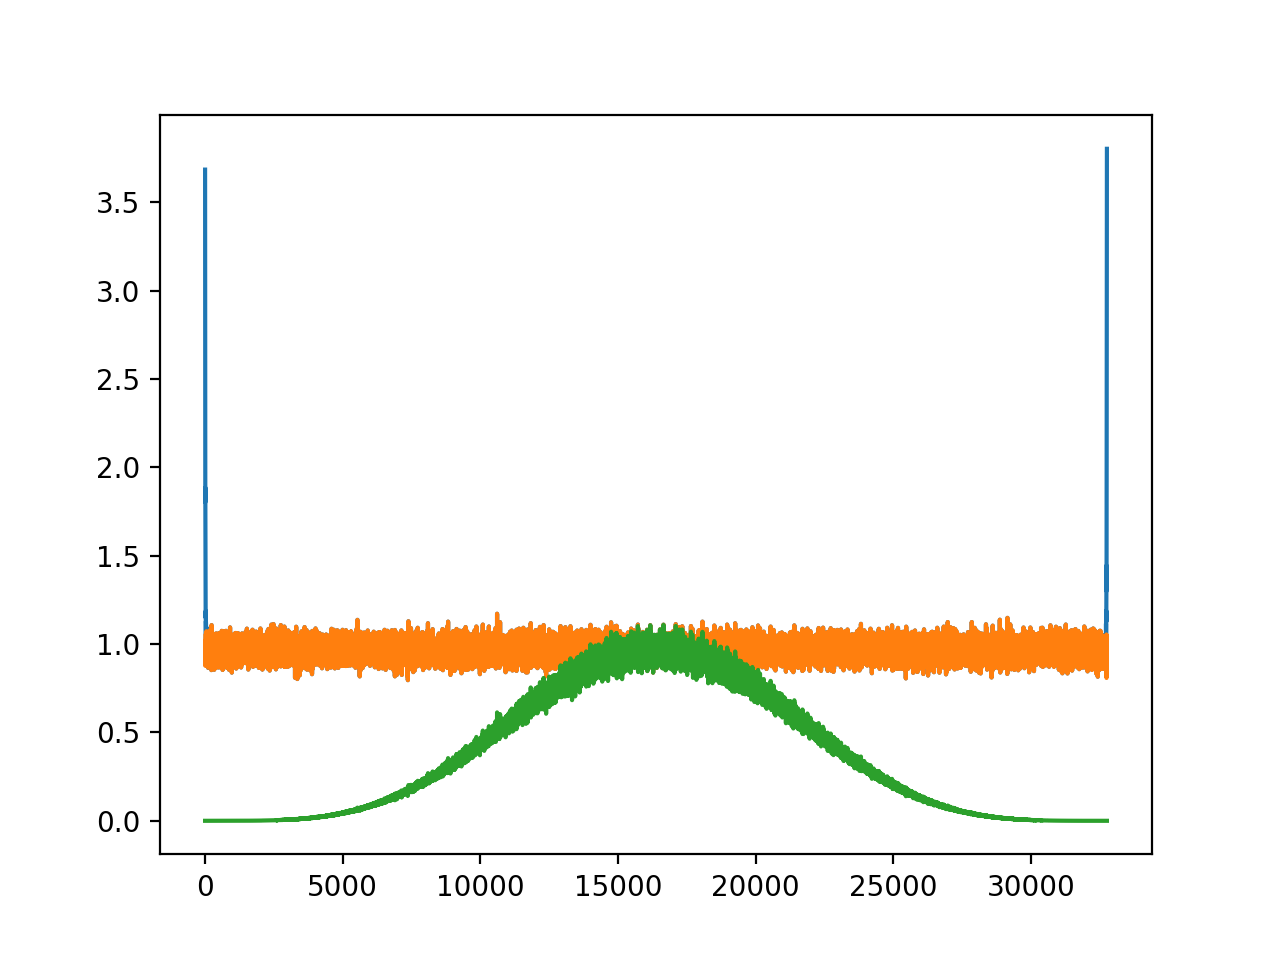
\includegraphics[width=3in]{plots/filtered_variance_5_3.png}
%  \caption{Stuff }
%  \label{fig:noise_sims}
%\end{figure}







%As shown in the appendix, non-stationary components of the
%noise can be equivalently treated as components of the solution, 




\subsection {Map Classes}

The generalized map is housed in an instance of the minkasi.Mapset
class.  Similar to the TodVec class, it containst a list of
generalized maps and assiacted methods to operate on those maps.
Crucially, it never access the contents of a map, except through
methods of the individual maps.  Key methods that the mapset relies on
include clear (assign zero to all parameters in the map), copy, dot
(sum the element-wise product of all parameters in two different map
instances of the same class), axpy (add a multiple of a second map to
a map), and \_\_add\_\_, \_\_sub\_\_, and \_\_mul\_\_, which do element-wise
additon, subtraction, and multiplication of two maps.  The wrapping of
the final three functions allows PCG to be written in a very natural
form.

In our experience, individual maps tend to fall into two broad
categories.  The first is maps of the sky (either explicitly maps, or
parameterized models of the sky such as point source fluxes).  All
TODs in principle could see such maps, and hence communication between
nodes is required to correctly handle these maps.  An entry in a
mapset for one of these maps then corresponds to a single (possibly
polarized) map of the sky.  Since minkasi assumes that data can be
kept in RAM, it also assumes that the mapping from timestream samples
to map pixels can also be kept in RAM.  As a result, the default
behavior is to use astropy.wcs to precompute the pixel mapping and
handle FITS header writing, so minkasi should work with essentially
all pixellizations supported by astropy.wcs.  HEALPix maps are also
supported as a special case via the healpy module.  

The second category is that of TOD-specific nuisance parameters, such
as data jumps and cut samples.  These maps tend to have a separate
entry for each TOD, and often share many methods in common.  To
accomodate this, there is a minkasi.tsModel class that corresponds to a
timestream-based model for a map (in particular, these maps tend to
not refer to the celestial pointing of samples), and each TOD has an
entry within the tsModel instance, which in turn is a single entry in
a mapset.  Because many of the methods are the same for different
timestream models, there is a generic class (minkasi.tsGeneric) that
new models can use as a base class.  If the parameters corresponding
to a desired set of timestream models can be represented by a numpy
array, then a new timestream-based model can often be added just by
writing an init function, and the pair of functions that go from data
to parameters and vice versa.  Timestream based models that exist in
minkasi include cut samples, and aribtrary timestream vectors (including
polynomials as a special case).  Minkasi can be used as a destriper by
setting the arbitrary vectors to destriping offsets and using a white
noise model for the detectors.  Sharp spectral lines can be modelled
by setting the arbitray vectors to sines/cosines at the line
frequency, or in the case of a line with time-varying amplitude, a few
sine/cosine at and near the line center.  


\subsection{Projection Operations}

Key to any mapmaker is the operator that map parameters into simulated
data and the transpose of that operator.  By default, these methods
are called map2tod and tod2map in minkasi.  As the names suggest, they
typically project a single map onto one TOD and vice versa.  The
low-level methods are associated with a map class since a TOD does not
know how it will be used, but a map should know how to handle data.
However, 


\subsection{Priors}
Frequently we have {\textit{some}} idea of what map parameters should
be, and being able to include this information while mapping can be
very powerful.  This can take many forms, from actual prior knowledge
of what a map should look like to handling non-stationary noise
components.  

For computational tractability, we restrict ourselves to
Gaussian likelihoods for the priors.  With this assumption, we add a
term to $\chi^2$ based on the map parameters and their expected values
and errors, leaving $\chi^2$ as follows:
\begin{eqnarray}
\label{eqn:prior_chisq}
\chi^2 = \left (d-\mathrm{A}m)^T \right ) \mathrm{N}^{-1} \left
(d-\mathrm{A}m \right ) + \left (\mathrm{H}m - p \right )^T \mathrm{Q}^{-1}
\left (\mathrm{H}m - p \right )
\end{eqnarray}
.  The first component of $\chi^2$ is unchanged from previous
discussions, $p$ is the vector of values we expect the map parameters
$m$ to agree with, $\mathrm{Q}$ is the associated noise matrix for $p$, and
$\mathrm{H}$ is a matrix that transforms $m$ into the native space of
$p$.  Often, but not always, $\mathrm{H}$ will not be present (or
equivalently, the identity matrix), and/or $p$ will be zero.  With the
prior included, the mapmaking equation becomes:
\begin{eqnarray}
\label{eqn:mapmaking_prior}
\left ( \mathrm{A}^T \mathrm{N}^{-1} \mathrm{A} + \mathrm{H}^T
\mathrm{Q}^{-1} \mathrm{H} \right ) m = \mathrm{A}^{T} \mathrm{N}^{-1}
d + \mathrm{H}^T \mathrm{Q}^{-1} p
\end{eqnarray}
We can use the conjugate gradient machinery we already have to solve
these equations simply by adding $\mathrm{H}^T \mathrm{Q}^{-1} p$ to
the dirty map, and adding $\mathrm{H}^T \mathrm{Q}^{-1} \mathrm{H}m $
to $ \mathrm{A}^T \mathrm{N}^{-1} \mathrm{A}m$ at each iteration of
PCG. 

We now provide some examples showing the utility and flexibility of
using priors in mapping.

\subsubsection{Pixellization Artifacts}
Representing a continuous map of the sky by piecewise-constant map
pixels can have some surprising effects, especially in the presence of
non-white noise.  One example is streaks or bowls around bright
sources (see xxx Naess) and suppression of point source flux.  These
effects arise from the mismatch between the smooth data and the
piecewise-constant model inferred from the pixellized map.  One way of
treating such effects (xxx see various ACT references) is to find
point sources in the map, directly model the timestreams given
telescope beams, and subtract the model timestreams from the data.
This approach can work well, but does not naturally handle pointing
errors in the data or bright sky structures more complicated than
simple point soruces.  An alternative approach is to say that the
noise in the timestreams picks up an additive component set by the
gradient in the map across a pixel.  Essentially, this lets
the mapper know that areas with large gradients will be hard to model,
and that the sky map should not try to marginally improve the fit over
bright, strongly pixellated areas at the expense of poorer fits in
nearby low-gradient areas.  

As originally developed, this technique, the Pixel Noise Generalized
Least Squares estimator (XGLS xxx Piazzo 2017), required running a
nested conjugate-gradient solver to handle the non-stationary noise at
each iteration of the mapping conjugate gradient solver.  Instead of
paying the steep computational price of nested conjugate gradient
iterations, minkasi solves for the pixellization noise with a prior
set by the gradient from preliminary maps.  Since the mean signal from
pixellization should be zero, we can set $p=0$ in Equation
\ref{eqn:mapmaking_prior}.  Similarly, since the prior is on
timestream samples and there is no mixing/remapping of the different
per-sample offsets, we can drop $\mathrm{H}$ and set $\mathrm{Q}$ to
be a diagonal matrix.  The entries of $\mathrm{Q}$ are just the square
of the map gradient associated with each timestream samples.  For the
common case where only a small fraction of the map has large enough
gradients to warrent the per-sample modelling, the impact on run-time
is only at the percent level.  Even in the worst-case scenario where
the entire map has large gradients and every sample must be modelled,
the impact time per conjugate gradient iteration would still only be
in the tens of percent, since the extra work required is linear in the
data, as opposed to the $n\log(n)$ scaling for the Fourier
transforms.  

xxx - can I add CBASS example here?

\subsubsection{Multi-Experiment Mapping}

Another case where adding a prior to the mapper can be useful is the
case of combining data at the same frequency from different
experiments.  The experiments could have different (but overlapping)
sky coverage, different beams, and different noise properties.  A
typical case would be observations of a galaxy cluster that combine
large-area low-resolution data (such as from Planck or ACT) with
small-area, high-resolution Mustang data.  Scales larger than a few
arcminutes will predominantly come from the large-area experiment
while smaller scales will come from Mustang.  In these sorts of cases,
a reasonable and useful assumption is that the large-scale data can be
described with a map-based likelihood over the region of interest, as
the map noise is relatively stationary on degree scales.  

In principle, a fully map-based combination is possible, but in
practice that is challenging since the small-area noise will vary over
the combined region.  A better alternative is to make a map of the
small-scale data that is consistent with the large-scale map.  We can
do this using a prior on the small-scale map.  If the beams of the
high- and low-resolution experiments are $\mathcal{B}_h$ and
$\mathcal{B}_l$ respectively, then for a high-resolution map $m$, the
low-resolution experiment would see $\mathcal{B}_l \ast
\mathcal{B}_h^{-1} \ast m$ where $\mathcal{B}_h^{-1}$ is understood to
be the the inverse of the beam when described in Fourier/spherical
harmonic space.  Normally these deconvolutions are unstable, but the
combination $\mathcal{B}_l \ast \mathcal{B}_h^{-1}$ will generally be
well defined, because the low-resolution beam goes to zero at high-$k$
faster than the high-resolution beam.  The low-resolution pixels will
almost certainly be larger than the high-resolution pixels
(\textit{e.g.} ACT uses 30'' pixels and Mustang 2''), and so we will
further need a binning/gridding operator $\mathrm{G}$ that averages
the high-resolution map pixels to match the low-resolution
pixellization.  

Under these assumptions, we can now predict the map the low-resolution
experiment should have seen $m_{l,p}$ given the high-resolution map
$m$:
\begin{eqnarray}
m_{l,p}=\mathrm{G} \mathcal{B}_l \mathcal{B}_h^{-1} m
\end{eqnarray}
.  We can now calculate a joint likelihood for the two experiments,
with the observed low-resolution map $m_l$, the low-resolution map
noise covariance $\mathrm{Q}$ and the mapping between low/high
resolution maps $\mathrm{H} \equiv \mathrm{G} \mathcal{B}_l
\mathcal{B}_h^{-1}$.  This now leaves $\chi^2$ in the form of Equation
\ref{eqn:prior_chisq} and we can solve for the joint map by solving
Equation \ref{eqn:mapmaking_prior}.  



%\subsubsection{Nonlinear Fitting} xxx



\appendix
\section{Equivalence of Marginalization and Solving for Nuisance Parameters}
In this appendix, we show that fitting for nuisance
parameters and including them in the noise matrix are mathematically
identical. 
% While one could, with pain, write down the proof
%analytically, it is straightforward to show it numerically in the case
%of a linear model.  
Without loss of generality, we can assume that the
noise matrix is the identity matrix, and that the prior is diagonal.
If they are not, then one can rotate into a space in which they are,
first using the Cholesky decomposition of the noise matrix, and then
the eigenvector/SVD matrix of the Cholesky-rotated prior.  We then are
trying to solve two different cases:
\begin{eqnarray}
\label{eqn:data_model}
\left (\mathrm{A}^T \left (\mathrm{I+Q} \right )^{-1} \mathrm{A}
\right ) m = \mathrm{A}^T\left (\mathrm{I+Q} \right )^{-1} d
\end{eqnarray}
\begin{eqnarray}
\left (\mathrm{A'}^T  \mathrm{A'} +\mathrm{Q'}^{-1} \right ) m' = \mathrm{A'}^T  d
\end{eqnarray}
Where, in the limit that we have one nuisance parameter per data
point, we have $\mathrm{A}' \equiv \left [\mathrm{A}\ \mathrm{I}\right ]$
 is the horizontal concatenation of
$\mathrm{A}$ with the identity matrix ({\textit{i.e.}} we are solving
for one extra parameter per data point, and that parameter corresponds
to an offset for that data point only).  The matrix $\mathrm{Q}'^{-1}$
has zeros along the diagonal corresponding to the actual fit
parameters (corresponding to no prior on those parameters), then
$\mathrm{Q}^{-1}$ along the rest of the diagonal.  Assuming the
various matrices are invertible, we can then solve
for a set of weights that, when applied to the data, give us our fit
parameters. In the first case, we have 
\begin{eqnarray}
m=\left (\mathrm{A}^T \left (\mathrm{I+Q} \right )^{-1}
\mathrm{A}\right )^{-1}\mathrm{A}^T\left (\mathrm{I+Q} \right )^{-1}d
\end{eqnarray}
or 
\begin{eqnarray}
\label{eqn:weights}
  W=\left(\mathrm{A}^T \left (\mathrm{I+Q} \right
  )^{-1}\mathrm{A}\right )^{-1}\mathrm{A}^T\left (\mathrm{I+Q} \right
  )^{-1}
\end{eqnarray}
For the second case, we have:
\begin{eqnarray}
m'=\left (\mathrm{A'}^T  \mathrm{A'} +\mathrm{Q'}^{-1} \right )^{-1}
\mathrm{A'}^T d
\end{eqnarray}
or
\begin{eqnarray}
  W'=\left (\mathrm{A'}^T  \mathrm{A'} +\mathrm{Q'}^{-1} \right
  )^{-1}\mathrm{A'}^T
\end{eqnarray}
We can carry out the matrix inversion by partitioning (which allows us
to replace primed matrices by unprimed ones).  Furthermore,
since we only care about the weights corresponding to the non-nuisance
parameters, we only need to calculate the upper two blocks of the
partitioned inverse.  We then have:
\begin{equation}
W'=\left [ \left (\mathrm{A}^T\mathrm{A}-\mathrm{A}^T(\mathrm{I}+\mathrm{Q}^{-1})\mathrm{A} \right )^{-1}  \ \ -\left
  (\mathrm{A}^T\mathrm{A}-\mathrm{A}^T (\mathrm{I}+\mathrm{Q}^{-1})^{-1}\mathrm{A}\right )^{-1} \mathrm{A}^T (\mathrm{I}+\mathrm{Q}^{-1})^{-1} \right ]
\left [ \mathrm{A} \ \ \mathrm{I} \right ]^T
\end{equation}
We can now carry out the matrix multiplication, group similar terms,
and insert copies of the identity matrix as needed to rewrite this as:
\begin{equation}
W'=\left (\mathrm{A}^{T} \left (\mathrm{I}-(\mathrm{I}+\mathrm{Q}^{-1})^{-1} \right
)\mathrm{A} \right )^{-1}\mathrm{A}^T 
\left (\mathrm{I}-(\mathrm{I}+\mathrm{Q}^{-1})^{-1} \right )
\end{equation}
Now, since $\mathrm{I}$ and $\mathrm{Q}$ are diagonal, we can simplify
$\left (I-(I+Q^{-1})^{-1} \right )$:
\begin{equation} 
\left (1-\frac{1}{1+\frac{1}{q}} \right ) = 1-\frac{q}{1+q} =
\frac{1+q}{1+q}-\frac{q}{1+q} = \frac{1}{1+q}
\end{equation}
So, we have 
\begin{equation}
\left (I-(I+Q^{-1})^{-1} \right ) = \left
(\mathrm{I}+\mathrm{Q} \right )^{-1}
\end{equation}
and we are left with a simplified expression for the weights:
\begin{equation}
W'=\left (\mathrm{A}^{T} (\mathrm{I}+\mathrm{Q})^{-1} \mathrm{A}
\right )^{-1} \mathrm{A}^T (\mathrm{I}+\mathrm{Q})^{-1}
\end{equation}
This is identical to Equation \ref{eqn:weights}, the weights for
putting the nuisance parameters into the noise, and so the two
approaches will produce identical answers for any data.  Thus, we have
complete freedom to choose between adding terms into the noise matrix,
or solving for the additional terms while adding a prior to their
values.

%A'*(I-inv(I+inv(\mathrm{Q})))*A)*A

%One then takes the first $n_{parameter}$ rows of $W'$, which
%correspond to the non-nuisance parameters, and then compares them to $W$.
%With random values for $\mathrm{A}$ and $\mathrm{Q}$, it is
%straightforward to show that these weights are the same, which means
%the recovered fit parameters will be identical if we put nuisance
%parameters in the noise, or solve for them with a prior. 

\end{document}
